\documentclass[border=4pt]{standalone}
\usepackage{tikz}
\usetikzlibrary{arrows.meta,calc,shapes.geometric}

\begin{document}
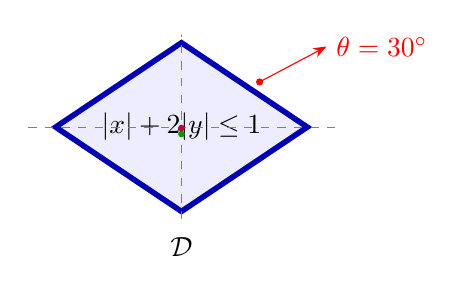
\begin{tikzpicture}[>=Stealth]
  \node[diamond,aspect=1.5,draw=blue!70!black,line width=2pt,fill=blue!7,
    minimum width=34mm,minimum height=22mm,inner sep=3pt,
    outer xsep=7pt,outer ysep=2pt] (d) at (0,0) {$|x|+2|y|\le1$};

  \draw[dashed,gray] (d.west) -- (d.east);
  \draw[dashed,gray] (d.south) -- (d.north);
  \fill[red] (d.30) circle (1.3pt);
  \draw[red,->] (d.30) -- ++(0.85,0.45) node[right] {$\theta=30^\circ$};
  \fill[green!60!black] (d.base) circle (1.2pt);
  \fill[purple] (d.mid) circle (1.2pt);
  \node[below=3pt] at (d.south) {$\mathcal D$};
\end{tikzpicture}
\end{document}
